% Template para la realización de la Presentacion de la Tesis.

% Tipo de Documento.
\documentclass[a4paper]{article}

% Idioma.
\usepackage[utf8x]{inputenc}
\usepackage[spanish]{babel}
\usepackage{babelbib}

% Margenes.
\usepackage[outer=4cm,inner=2cm,top=2cm,bottom=2cm]{geometry}
\usepackage{fancyhdr}
\usepackage{lastpage}

% Graficos.
\usepackage{graphicx}
\graphicspath{{./images/}}

% Codigo Fuente.
\usepackage{tabularx}

% Hypervinculos.
\usepackage{url}
\usepackage{color,hyperref}
\definecolor{black}{rgb}{0.0,0.0,0.0}
\definecolor{darkblue}{rgb}{0.0,0.0,0.3}
\hypersetup{colorlinks,breaklinks,
            linkcolor=black,urlcolor=darkblue,
            anchorcolor=darkblue,citecolor=darkblue}

% Guiones
\hyphenation{pro-ble-ma}
\hyphenation{ge-ne-ra-ra}
\hyphenation{pos-te-rior-men-te}

% Definicion de la hoja de firmas.
\newcommand{\signature}[7]{
	\vfill

	\begin{flushright}
		#1, \today
	\end{flushright}
	\vspace{3cm}

	\noindent
	\centering
	\begin{tabularx}{0.9\textwidth}{cXc}
		\multicolumn{3}{c}{\rule{5cm}{1pt}}\\
		\multicolumn{3}{c}{#2}\\
		\multicolumn{3}{c}{#3}\\
		\vspace{3cm}\\
		\rule{5cm}{1pt} & \hspace{2.5cm} & \rule{5cm}{1pt} \\
		#4 & ~ & #5 \\
		#6 & ~ & #7
	\end{tabularx}
	\vspace{1cm}
}

% Encabezado y Titulo del Documento y de la Tesis.
\title{
	{\normalsize
		Universidad de Buenos Aires\\
		Facultad de Ingeniería -- Departamento de Electrónica\\
		Propuesta de Tesis de Ingeniería Electrónica\\
		\vspace{0.7cm}
	}
	Diseño, validación e implementación de una arquitectura RISC
}

% Datos de autor: Tesista, Director y Co-director.
\author{	\textbf{Tesista}															\\
			Luciano César Natale, \textit{Padrón Nro. 86.659}               			\\
            \texttt{ \href{mailto:luchonat@gmail.com}{luchonat@gmail.com}}			\\[2.5ex]
            \textbf{Director}																\\
            Ing. Nicolás Álvarez, \textit{Profesor Adjunto}             				\\
            \texttt{ \href{mailto:nalvare2001@yahoo.com.ar}{nalvare2001@yahoo.com.ar}}  \\[2.5ex]
            \textbf{Co-director}															\\
            Ing. Octavio Alpago, \textit{JTP}               					\\
            \texttt{ \href{mailto:oalpago@gmail.com}{oalpago@gmail.com}}                \\[2.5ex]
       }

% Fecha.
\date{\today}

% Pie de Pagina.
\pagestyle{fancy}
\lhead{}
\chead{}
\rhead{}
\lfoot{}
\cfoot{
	{\footnotesize
	\emph{Diseño, validación e implementación de una arquitectura RISC}\\
	Plan de Tesis -- Página \thepage\ de \pageref{LastPage}
	}
}
\rfoot{}
\renewcommand{\headrulewidth}{0pt}
\renewcommand{\footrulewidth}{0.4pt}

% Documento.
\begin{document}

\maketitle

%\thispagestyle{empty}

%\begin{abstract}
%\end{abstract}

\thispagestyle{fancy}

\section{Objeto y área de la tesis}

El objetivo principal de este trabajo consiste en diseñar, validar e implementar una arquitectura RISC\footnote{\label{RISC} \emph{Reduced Instruction Set Computer}. Técnica de diseño de unidades de procesamiento basada en el hecho de que un conjunto de instrucciones simple provee una mayor performance al ser combinado con una arquitectura capaz de ejecutar dichas instrucciones en algunos pocos ciclos de máquina.}. El diseño incluirá la completa especificación funcional de la arquitectura y su conjunto de instrucciones. El diseño se validará mediante el desarrollo en software de un emulador de la arquitectura; la implementación se realizará en el lenguaje de descripción de hardware Verilog, y se sintetizárá en un dispositivo FPGA\footnote{\label{FPGA} \emph{Field Programmable Gate Array}. Dispositivo semiconductor que contiene bloques de lógica cuya interconexión y funcionalidad puede ser configurada `in situ' mediante un lenguaje de descripción especializado.}.

El interés en este desarrollo proviene de la necesidad de contar con un núcleo de procesamiento altamente configurable y suficientemente flexible y sencillo para distintas aplicaciones dentro del ámbito de la investigación en los Laboratorios de Microelectrónica y de Sistemas Embebidos; sintetizable en FPGA.

El área profesional de relevancia del trabajo de tesis es el diseño de sistemas digitales y su aplicación como base de proyectos de investigación que necesiten de un núcleo de procesamiento configurable y sencillo.

\newpage

\section{Introducción, antecedentes y actualidad}

Desde la aparición de los microprocesadores a mediados de los años 70, la tendencia fue el aumento de la complejidad de las arquitecturas, generando un efecto de ``bola de nieve'', al ir superponiendo capas sobre un núcleo central. Existió, entonces, una reacción adversa a esta tendencia. Por ejemplo, la arquitectura experimental de IBM 801; y también en Berkeley, Patterson y Ditzel fueron los primeros en acuñar el término RISC, para descibir una nueva clase de arquitectura que deshacía el camino del resto de las arquitecturas hasta el momento, conocidas, en contraposición, como CISC\footnote{\label{CISC} \emph{Complex Instruction Set Computer}. Técnica de diseño de unidades de procesamiento basadas en el hecho de que el conjunto de instrucciones debe ser lo más poderoso posible.}. A partir de este antecedente, los principales fabricantes de microprocesadores han lanzado al mercado sus propias implementaciones basadas en los principios establecidos en IBM y Berkeley.

El concepto de las arquitecturas RISC se basa, principalmente, en el hecho de que al simplificar la lógica necesaria para la ejecución de una instrucción permite aumentar la frecuencia de operación de las compuertas que componen la lógica. Además, es posible dividir la ejecución de las instrucciones en etapas sencillas y consecutivas, permitiendo de esta manera implementar fácilmente optimizaciones como, por ejemplo, una arquitectura de \emph{pipeline}\footnote{\label{Pipeline} Técnica de diseño de arquitecturas de computadoras en la que se segmenta la ejecución de las instrucciones en múltiples etapas, permitiendo que múltiples instrucciones estén ejecutándose en paralelo.}. Es por esto que el conjunto de instrucciones es sencillo, permitiendo solamente operaciones básicas entre registros internos del microprocesador. El trabajo realizado por cada instrucción, en general, es menor que el generado por una instrucción CISC, pero se hace de manera sencilla y rápida. Es importante notar que no solamente la ganancia radica en poder aumentar la frecuencia de operación de la lógica, sino que estas condiciones facilitan el desarrollo de diseños de bajo consumo, característica muy valorada en el nicho de los sistemas embebidos.

El mercado de los sistemas embebidos es excesivamente amplio y está inserto en todas las industrias. En un automóvil, por ejemplo, podemos encontrar microprocesadores en el sistema de frenos, en la central de inyección electrónica, en el sistema de entretenimiento y navegación, etc. La otra arista de vital importancia para el mercado de los sistemas embebidos, es el de los dispositivos móviles, donde se vuelve vital el requerimiento de bajo consumo. Estamos viviendo la revolución de IoT\footnote{\label{Internet of Things} Es un concepto que se refiere a la interconexión digital de objetos cotidianos con internet.}, que se trata básicamente de sistemas embebidos autónomos que estan conectados a ``la nube'' y pueden ser monitoreados y controlados remotamente a través de \emph{Internet}.

Dentro del universo de las arquitecturas RISC, actualmente se destacan dos: MIPS y ARM. La primera, fue desarrollada por un grupo de investigadores de la Universidad de Stanford (entre ellos John L. Hennessy, pionero del concepto RISC junto a David Patterson, coautores de la bibliografía más relevante del área). Esta arquitectura, por su sencillez, es la predilecta al momento del desarrollo de cursos enfocados en la enseñanza de arquitectura de computadoras. Si bien MIPS posee gran relevancia académica, es muy popular en el mercado de los microprocesadores en sistemas embebidos como equipos de telecomunicaciones, decodificadores de TV digital, y consolas de entretenimiento, con ejemplos muy conocidos como \emph{Nintendo} y \emph{PlaySation}. ARM, por otro lado, ha ganado una importante porción del mercado de los sistemas embebidos (con un gran aporte de los dispositivos móviles), basando su modelo de negocios en la venta de la propiedad intelectual (IP, \emph{intellectual property}) del diseño de los microprocesadores a las empresas que finalmente producen el microprocesador.

\section{Desarrollo previsto de la tesis}

\subsection{Teoría, enfoque y métodos a utilizar}

El enfoque de la tesis se basará en un desarrollo teórico del conjunto de instrucciones y de las características de la arquitectura; y en el desarrollo
práctico del emulador y la implementación en lenguaje descriptor de hardware.

El concepto central detrás del desarollo será el de \textbf{ortogonalidad}. Esto implica, por una parte, que los bloques constructivos de la arquitectura que se repiten sean independientes e indiferenciables entre sí. Por otra parte, los formatos de las instrucciones, en la medida de lo posible, se diseñaran de manera tal que se pueda mantener el mismo ancho de campo para los datos inmediatos y los desplazamientos (excepto en los casos donde es explícitamente conveniente agrandarlos sin penalizar la complejidad del diseño).

El objetivo perseguido va a ser el de mantener la sencillez y la ortogonalidad, favoreciendo así la simplificación de la implementación. Se trabajará en el desarrollo de la definición de la arquitectura y su conjunto de instrucciones en favor de este objetivo. Se definirá la interfaz física para la conectividad con periféricos, los tipos de datos que maneja la arquitectura, la cantidad y tipos de registros internos, el acceso a memoria de programa y de datos con su organización y modo de direccionamiento, la interfaz con la ALU\footnote{\label{ALU} \emph{Arithmetic Logic Unit}. Bloque constructivo encargado de realizar las operaciones aritmético lógicas sobre los datos.} y la FPU\footnote{\label{FPU} \emph{Floating Point Unit}. Bloque constructivo encargado de realizar las operaciones en punto flotante sobre los datos.}, mecanismos de manejos de excepeciones e interrupciones, modos de operación y manejo de periféricos. Luego se definirá el conjunto de instrucciones que ejecutará la arquitectura.

Una vez definida la arquitectura y su conjunto de instrucciones, se prodecerá a diseñar los vectores de prueba para poder validar las implementaciones. Se desarrollará un emulador de la arquitectura que deberá validar los vectores de prueba diseñados. Una vez concluida esta etapa, se implementará a nivel RTL el diseño en \emph{Verilog}. Este diseño será validado mediante simulaciones y utilizando dispositivos programables. Se validará también contra los vectores de prueba. Se analizarán los recursos utilizados en dispositivos FPGA. Se realizará un análisis comparativo entre la arquitectura desarrollada y otras arquitecturas RISC.

\subsection{Estudios conexos}

Asignaturas y otros estudios previstos o previos que son relevantes al desarrollo de la tesis:

\begin{itemize}
	\item \textbf{Sistemas digitales:} asignatura que abarca la teoría de técnicas de diseño de hardware digital y codificación de sistemas digitales, así como también su síntesis y medición.
	\item \textbf{Organización de computadoras:} asignatura en la cual se cubren los aspectos teóricos del diseño de arquitecturas.
\end{itemize}

\subsection{Alcance proyectado para la tesis}

Como resultados a obtener de la tesis se tienen los siguientes:

\begin{itemize}
    \item Especificación completa de la arquitectura
    \item Vectores de prueba
    \item Emulador de la arquitectura
    \item \emph{IP Core} codificado en el lenguaje \emph{Verilog} de la arquitectura completa
    \item Resultado de los vectores de prueba tanto en el emulador como en el \emph{IP Core}
    \item Análisis comparativo entre la arquitectura desarrollada y otras arquitecturas RISC
    \item Proposición de trabajos futuros y/o mejoras.
\end{itemize}

Para asegurar que el proyecto de tesis incluya todos los trabajos requeridos, los procesos a completar se describen en un plan de trabajo en la siguiente sección.

\newpage

\subsection{Plan de trabajo}

La duración total del trabajo se estima en un año y se considera que el mismo estará compuesto por las siguientes etapas:

\begin{itemize}
    \item \textbf{Investigación bibliográfica:} recolección de libros, \emph{papers}, trabajos de tesis, y fuentes de investigación con el objetivo de obtener el entendimiento teórico requerido y conocer el estado del arte en el tema a trabajar.
    \item \textbf{Introducción al trabajo de tesis:} comprender la teoría de las arquitecturas RISC. Describir el contenido teórico requerido para exponer los conceptos de funcionamiento del hardware a desarrollar.
    \item \textbf{Análisis de arquitecturas existentes:} analizar las diferentes arquitecturas existentes con sus pro y contras. Obtener de este análisis las relaciones de compromiso asumidas en ellas para poder aplicarlas en la arquitectura a desarrollar.
    \item \textbf{Diseño de la arquitectura y su conjunto de instrucciones:} realizar la especificación funcional de la arquitectura y su conjunto de instrucciones.
    \item \textbf{Validación:} desarrollar los vectores de pruebas que permitirán validar la arquitectura.
    \item \textbf{Emulación:} desarrollar el emulador de la arquitectura y validar los vectores de pruebas.
    \item \textbf{Implementación:} desarrollar el \emph{IP core} en un ambiente de simulación y, en la medida que sea posible, en campo. Realizar la síntesis del mismo para distintos dispositivos FPGA, medir recursos utilizados, máxima frecuencia de operación y potencia consumida. Validar los vectores de pruebas.
    \item \textbf{Conclusiones y trabajos a futuro:} se extraerán las conclusiones pertinentes sobre los resultados obtenidos y se propondrán, si correspondiese, futuras mejoras de la arquitectura.
    \item \textbf{Preparación del informe final:} se consolidará la documentación con la memoria de la tesis la cual contendrá el resultado de todo el trabajo realizado. Se revisará la tesis por el Director, Co-director y por los pares antes de enviarla al Jurado.
    \item \textbf{Preparación de la presentación y defensa de la tesis:} se elaborarán diapositivas para la presentación con los objetivos, alcance, introducción a las arquitecturas RISC, desarrollo de la arquitectura, resultados obtenidos, conclusiones y trabajos a futuro. La misma será posteriormente utilizada para la defensa.
\end{itemize}

En la figura \ref{fig:tabla_actividades} se encuentra el plan propuesto para la formación del tesista y el cumplimiento de los objetivos.

\begin{figure}[h!]
  \begin{center}
    %trim option's parameter order: left bottom right top
    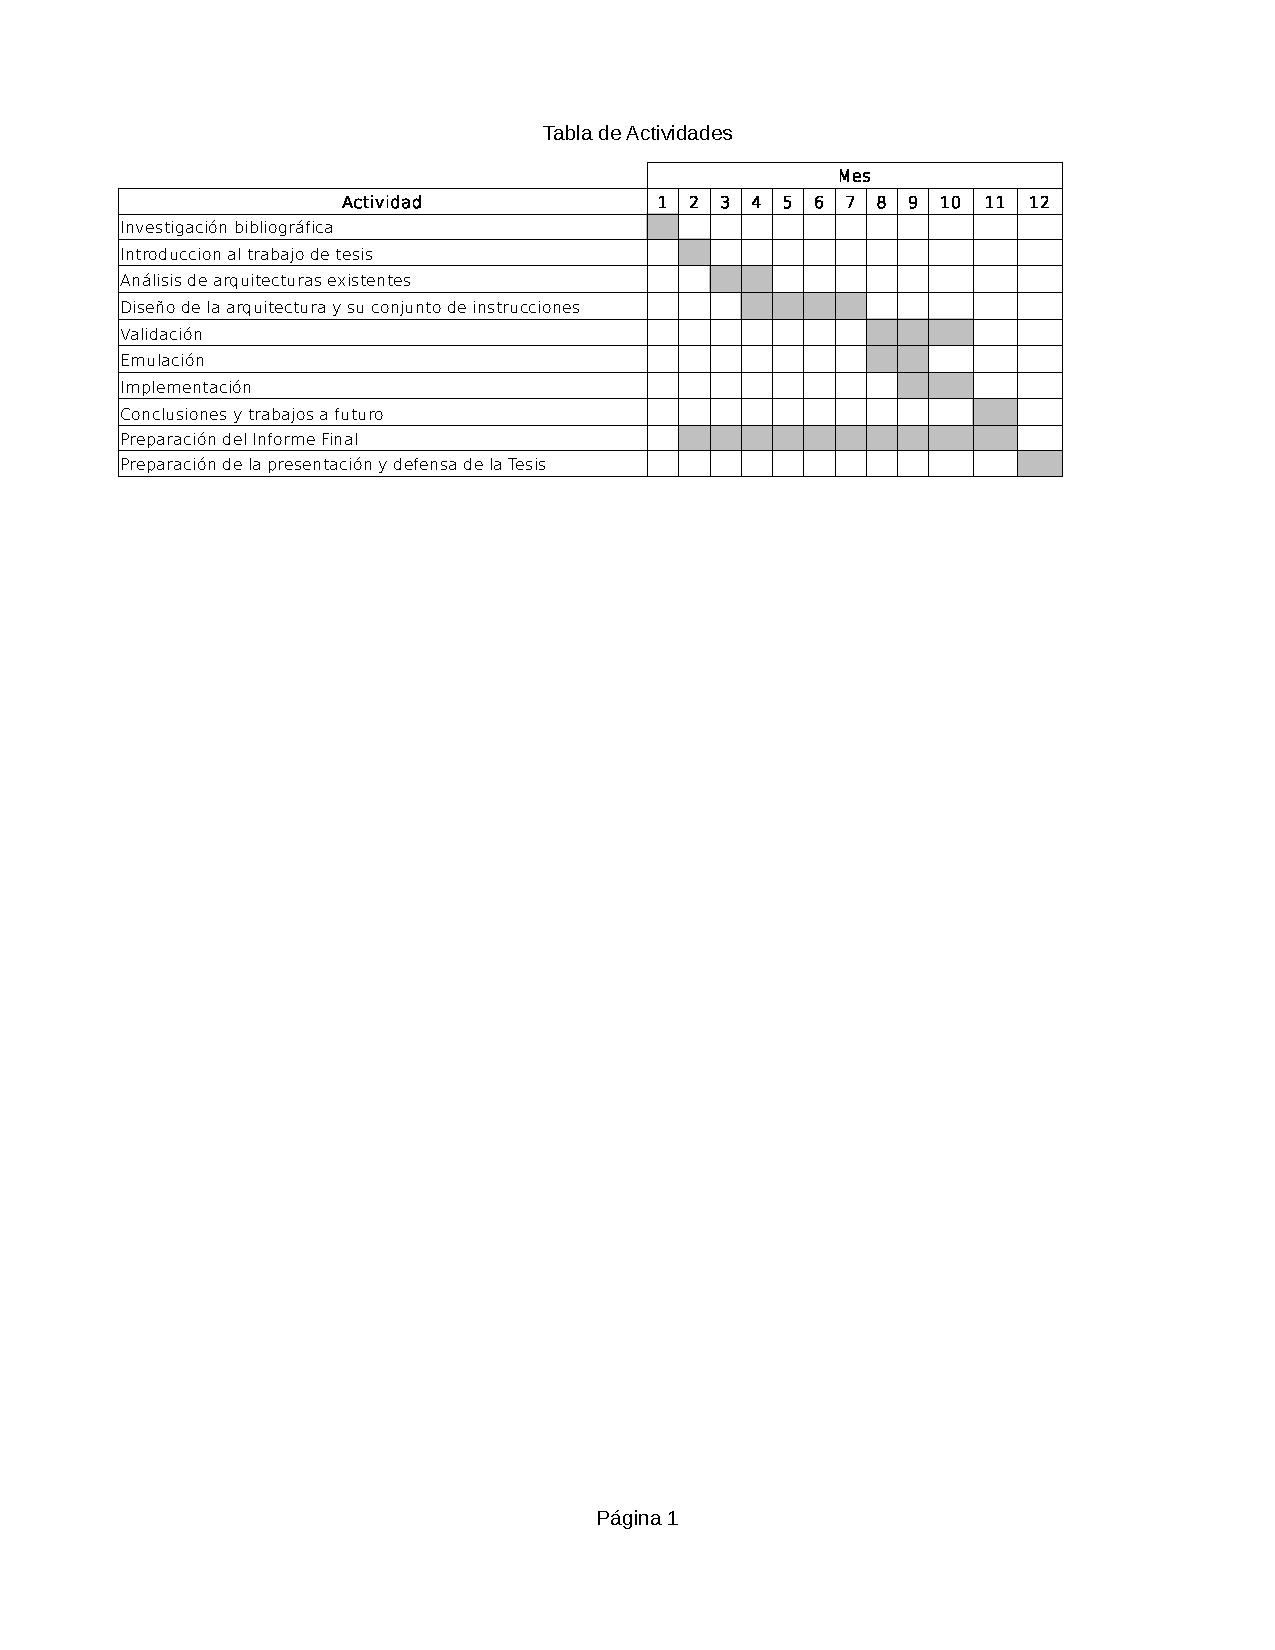
\includegraphics[trim = 20mm 180mm 20mm 25mm, clip, width=\textwidth]{tabla_actividades}
  \end{center}
  \caption{Diagrama de las actividades a realizar por el tesista.}
  \label{fig:tabla_actividades}
\end{figure}
	
\newpage

\section{Bibliografía}

\begin{thebibliography}{99}

\bibitem{Patterson - Hennessy} David A. Patterson \& John L. Hennessy, ``Computer Organization and Desing - The Hardware/Software Interface'', Fourth Edition - ARM Edition, Morgan Kaufmann, 2010.
\bibitem{Hennesy - Patterson} John L. Hennessy \& David A. Patterson, ``Computer Architecture - A Quantitative Approach'', Fourth Edition, Morgan Kaufmann, 2010.
\bibitem{Murdocca - Heuring} Miles J. Murdocca \& Vincent P. Heuring ``Principles of Computer Architecture'', First Edition, Prentice Hall, 1999.
\bibitem{Wakerly} John F. Wakerly, ``Diseño Digital - Principios y Prácticas'', Tercera Edición, Pearson, 2010.
\end{thebibliography}

\newpage

\signature{Buenos Aires}{Sr. Luciano César Natale}{Tesista}{Ing. Nicolás Álvarez}{Ing. Octavio Alpago}{Prof. Adjunto, Director}{JTP, Co-director}

\end{document}
